\documentclass{article}

\usepackage{amsmath,amsthm,amssymb}
\usepackage{commath}
\usepackage{mathtools}
\usepackage{enumerate}
\usepackage{subcaption}
\usepackage{float}
\usepackage{tikz}
\usepackage[margin=.8in]{geometry}
\usepackage{multicol}
\usepackage{epstopdf}
\usepackage[linesnumbered]{algorithm2e}

\newenvironment{algorithmic}{%
\renewenvironment{algocf}[1][h]{}{}% pass over the floating stuff
\algorithm
}{%
\endalgorithm
}

\usetikzlibrary{positioning, shapes, automata, arrows, backgrounds, shapes.geometric}

\setlength{\parindent}{0pt}
\setlength{\parskip}{8pt}

\usepackage[utf8]{inputenc}
\begin{document}
\title{Assignment 13 \\ Advanced Algorithms \& Data Structures PS}%
\author{Christian Müller 1123410 \\ Daniel Kocher, 0926293}%
\maketitle

{\bfseries Aufgabe 23}%

Finden Sie die optimale Klammerung f{\"u}r das Matrixkettenprodukt gegeben durch
die Folge von Dimensionen $(41, 40, 4, 25, 34, 12)$. Geben Sie alle $m[i, j]$
und $s[i, j]$ an.

$m[i, j]$ \ldots minimale Anzahl von Operationen zur Berechnung des Teilprodukts
$A_{i, \ldots, j}$.

$s[i, j]$ \ldots optimaler Splitwert $k$, f{\"u}r den das  Minimum angenommen
wird.

\begin{equation}
m[i, j] = \begin{cases}
  0, & \text{ falls } i = j \\
  \min\limits_{i \leq k < j} \left\{ m[i, k] + m[k + 1, j] + p_{i - 1}p_kp_j \right\}, & \text{ sonst}
\end{cases}
\end{equation}

\begin{equation}
P = \left\{ p_0 = 41, p_1 = 40, p_2 = 4, p_3 = 25, p_4 = 34, p_5 = 12 \right\}
\end{equation}

Aus $P$ kann man also entnehmen, dass wir $n = 5$ Matrizen multiplizieren wollen:
\begin{center}
\begin{tabular}{ll}
$A_1: 41 \times 40$ & $A_4: 25 \times 34$ \tabularnewline
$A_2: 40 \times 4$ & $A_5: 34 \times 12$ \tabularnewline
$A_3: 4 \times 25$ & \tabularnewline
\end{tabular}
\end{center}

Zur Ermittlung der optimalen Klammerung sowie aller Werte f{\"u}r $m[i, j]$ bzw.
$s[i, j]$, wenden wir nun den dynamischen Algorithmus $dyn-mat-ket$ und den
rekursiven Algorithmus $Opt-Klam$ an. Im Folgenden sind die Ergebnisse f{\"u}r
$m[i, j]$ (Table~\ref{tbl:m}) bzw. $s[i, j]$ (Table~\ref{tbl:s}) zusammengefasst.
Darunter sind die Berechnungsschritte angegeben (die ersten wurden weggelassen,
da ohnehin immer der berechnete Wert bleibt, da das $\min$ mit $\infty$ gebildet
wird). Die fett markierten Werte sind jene, die in $m[i, j]$ bzw. $s[i, j]$
eingetragen wurden.

\begin{minipage}{.45\textwidth}
\begin{table}[H]
  \centering
  \begin{tabular}{|l|l|l|l|l|l|}
  \hline
  $j$ \textbackslash $i$  & $1$     & $2$     & $3$     & $4$     & $5$ \tabularnewline
  \hline\hline
  $5$                     & $13560$ & $6952$  & $5032$  & $10200$ & $0$ \tabularnewline
  \hline
  $4$                     & $15536$ & $8840$  & $3400$  & $0$     & -   \tabularnewline
  \hline
  $3$                     & $10660$ & $4000$  & $0$     & -       & -   \tabularnewline
  \hline
  $2$                     & $6560$  & $0$     & -       & -       & -   \tabularnewline
  \hline
  $1$                     & $0$     & -       & -       & -       & -   \tabularnewline
  \hline\hline
  \end{tabular}
  \caption{$m[i, j]$ f{\"u}r $1 \leq i, j \leq 5$.}
  \label{tbl:m}
\end{table}
\end{minipage}
\begin{minipage}{.45\textwidth}
\begin{table}[H]
  \centering
  \begin{tabular}{|l|l|l|l|l|l|}
  \hline
  $j$ \textbackslash $i$  & $1$ & $2$  & $3$  & $4$ \tabularnewline
  \hline\hline
  $5$                     & $2$ & $2$  & $4$  & $4$ \tabularnewline
  \hline
  $4$                     & $2$ & $2$  & $3$  & -   \tabularnewline
  \hline
  $3$                     & $2$ & $2$  & -    & -   \tabularnewline
  \hline
  $2$                     & $1$ & -    & -    & -   \tabularnewline
  \hline\hline
  \end{tabular}
  \caption{$s[i, j]$ f{\"u}r $1 \leq i \leq 4$ und $2 \leq j \leq 5$.}
  \label{tbl:s}
\end{table}
\end{minipage}

\clearpage

\begin{equation}
m[1, 3] = \min\limits_{1 \leq k < 3} \left\{ m[1, k] + m[k + 1, 3] + p_0p_kp_3 \right\}
\end{equation}

\begin{equation}
m[1, 3] = \min\begin{cases}
  m[1, 1] + m[2, 3] + p_0p_1p_3 = 0 + 4000 + 41000 = 45000 (k = 1)\\
  m[1, 2] + m[3, 3] + p_0p_2p_3 = 6560 + 0 + 4100 = \textbf{10660 (k = 2)}
\end{cases}
\end{equation}

\begin{equation}
m[2, 4] = \min\limits_{2 \leq k < 4} \left\{ m[2, k] + m[k + 1, 4] + p_1p_kp_4 \right\}
\end{equation}

\begin{equation}
m[2, 4] = \min\begin{cases}
  m[2, 2] + m[3, 4] + p_1p_2p_4 = 0 + 3400 + 5440 = \textbf{8840 (k = 2)} \\
  m[2, 3] + m[4, 4] + p_1p_3p_4 = 4000 + 0 + 34000 = 38000 (k = 3)
\end{cases}
\end{equation}

\begin{equation}
m[3, 5] = \min\limits_{3 \leq k < 5} \left\{ m[3, k] + m[k + 1, 5] + p_2p_kp_5 \right\}
\end{equation}

\begin{equation}
m[3, 5] = \min\begin{cases}
  m[3, 3] + m[4, 5] + p_2p_3p_5 = 0 + 10200 + 1200 = 11400 (k = 3) \\
  m[3, 4] + m[5, 5] + p_2p_4p_5 = 3400 + 0 + 1632 = \textbf{5032 (k = 4)}
\end{cases}
\end{equation}

\begin{equation}
m[1, 4] = \min\limits_{1 \leq k < 4} \left\{ m[1, k] + m[k + 1, 4] + p_0p_kp_4 \right\}
\end{equation}

\begin{equation}
m[1, 4] = \min\begin{cases}
  m[1, 1] + m[2, 4] + p_0p_1p_4 = 0 + 8840 + 55760 = 64600 (k = 1) \\
  m[1, 2] + m[3, 4] + p_0p_2p_4 = 6560 + 3400 + 5576 = \textbf{15536 (k = 2)} \\
  m[1, 3] + m[4, 4] + p_0p_3p_4 = 10660 + 0 + 34850 = 45510 (k = 3)
\end{cases}
\end{equation}

\begin{equation}
m[2, 5] = \min\limits_{2 \leq k < 5} \left\{ m[2, k] + m[k + 1, 5] + p_1p_kp_5 \right\}
\end{equation}

\begin{equation}
m[2, 5] = \min\begin{cases}
  m[2, 2] + m[3, 5] + p_1p_2p_5 = 0 + 5032 + 1920 = \textbf{6952 (k = 2)} \\
  m[2, 3] + m[4, 5] + p_1p_3p_5 = 4000 + 10200 + 12000 = 26200 (k = 3) \\
  m[2, 4] + m[5, 5] + p_1p_4p_5 = 8840 + 0 + 16320 = 25160 (k = 4)
\end{cases}
\end{equation}

\begin{equation}
m[1, 5] = \min\limits_{1 \leq k < 5} \left\{ m[1, k] + m[k + 1, 5] + p_0p_kp_5 \right\}
\end{equation}

\begin{equation}
m[1, 5] = \min\begin{cases}
  m[1, 1] + m[2, 5] + p_0p_1p_5 = 0 + 6952 + 19680 = 26632 (k = 1) \\
  m[1, 2] + m[3, 5] + p_0p_2p_5 = 6560 + 5032 + 1968 = \textbf{13560 (k = 2)} \\
  m[1, 3] + m[4, 5] + p_0p_3p_5 = 10660 + 10200 + 12300 = 33160 (k = 3) \\
  m[1, 4] + m[5, 5] + p_0p_4p_5 = 15536 + 0 + 16728 = 32264 (k = 4)
\end{cases}
\end{equation}

\clearpage

Damit ergibt sich nach Aufruf von $Opt-Klam(A, s, 1, n)$ folgende optimale
Klammerung:
$\left( \left( A_1 \right) \left( A_2 \right) \right) \left( \left( \left( A_3 \right) \left( A_4 \right) \right) \left( A_5 \right) \right)$.

Mit dieser Klammerung ergeben sich die minimalen Kosten von $13560$:

\begin{equation}
A' = A_1 \cdot A_2 \Rightarrow (41 \times 40)\text{-Matrix} \cdot (40 \times 4)\text{-Matrix} = 41 \cdot 40 \cdot 4 = 6560 \quad (41 \times 4)\text{-Matrix}
\end{equation}

\begin{equation}
A'' = A_3 \cdot A_4 \Rightarrow (4 \times 25)\text{-Matrix} \cdot (25 \times 34)\text{-Matrix} = 4 \cdot 25 \cdot 34 = 3400 \quad (4 \times 34)\text{-Matrix}
\end{equation}

\begin{equation}
A''' = A'' \cdot A_5 \Rightarrow (4 \times 34)\text{-Matrix} \cdot (34 \times 12)\text{-Matrix} = 4 \cdot 34 \cdot 12 = 1632 \quad (4 \times 12)\text{-Matrix}
\end{equation}

\begin{equation}
A'''' = A' \cdot A''' \Rightarrow (41 \times 4)\text{-Matrix} \cdot (4 \times 12)\text{-Matrix} = 41 \cdot 4 \cdot 12 = 1968 \quad (41 \times 12)\text{-Matrix}
\end{equation}

Damit ergeben sich die Gesamtkosten dieser Klammerung mit $6560 + 3400 + 1632 + 1968 = \textbf{13560}$.

Rekursion $Opt-Klam(A, s, 1, n)$ :
\begin{figure}[H]
  \centering
\begin{subfigure}[b]{.45\textwidth}
    \centering
    $X \cdot Y=(A_1A_2)((A_3A_4)A_5)$
    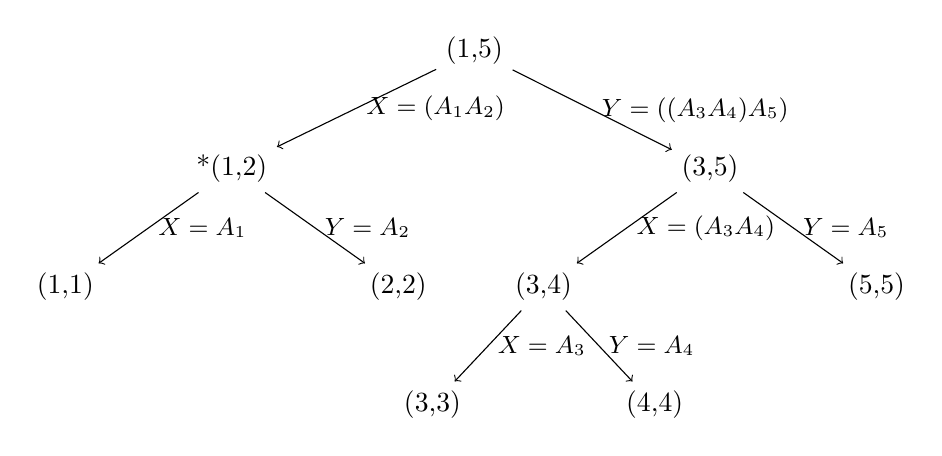
\begin{tikzpicture}
      \node { (1,5) }
      	child { node [left = 5em] { *(1,2)  }  
        child { node [left = 2.5em] { (1,1) }
        edge from parent [->] node[right] {\small $X=A_1$} }       	 
        child { node [right = 2.5em] { (2,2)  }
        edge from parent [->] node[right] {\small $Y=A_2$} }
        edge from parent [->] node[right] {\small $X=(A_1A_2)$}
      }
      	child { node [right = 5em] { (3,5)  } 
        child { node [left = 2.5em] { (3,4) }
        child { node [left = .5em] { (3,3) }
   		edge from parent [->] node[right] {\small $X=A_3$} }
        child { node [right = .5em] { (4,4)} 
        edge from parent [->] node[right] {\small $Y=A_4$}}
         edge from parent [->] node[right] {\small $X=(A_3A_4)$}}       	 
        child { node [right = 2.5em] { (5,5) }
        edge from parent [->] node[right] {\small $Y=A_5$} } 
        edge from parent [->] node[right] {\small $Y=((A_3A_4)A_5)$}
      };
      
    \end{tikzpicture}
    \label{subfig:aufg9-i-1-after}
    \caption{Ende}
  \end{subfigure}
\end{figure}
*: bedeutet $Opt-Klam(A, s, 1, n)$ \\
$X=Opt-Klam(A,s,1,s[1,2]=1)=A_1$\\
$Y=Opt-Klam(A,s,s[1,2]+1=2,2)=A_2$\\
Return $(XY)$
\end{document}
